\chapter {RESULTS AND DISCUSSION}
\hspace{0.5cm}
This chapter presents and analyzes the results obtained from the proposed system, the AI-Powered Code Documentation Generator. The system was evaluated using source code files provided through two input methods: direct file uploads via the web interface and repository-based inputs through public Git URLs. This dual-mode testing ensured that the system was assessed under both isolated and real-world development scenarios.

The results demonstrate that the system is capable of effectively processing multi-language codebases and generating well-structured, coherent and contextually relevant documentation. By integrating techniques such as syntactic analysis, structural feature extraction and language model-based generation, the system successfully transforms raw source code into meaningful documentation. Overall, the observed outputs highlight the system’s reliability, scalability and practical applicability in automating documentation tasks across diverse programming environments..

\section{Results}
\hspace{0.5cm}The system was tested in different input modes to evaluate its functionality and output quality. The following figures illustrate the working of the system and the documentation generated at various stages.
\par The screenshot in Figure 7.1 displays the homepage of the AI-Powered Code Documentation Generator when in file upload mode. There are two modes in which a user can input the source code. These modes are Upload Files and Repository URL.
\vspace{1cm}
\FloatBarrier
\begin{figure}[h]
	\centering
	\fbox{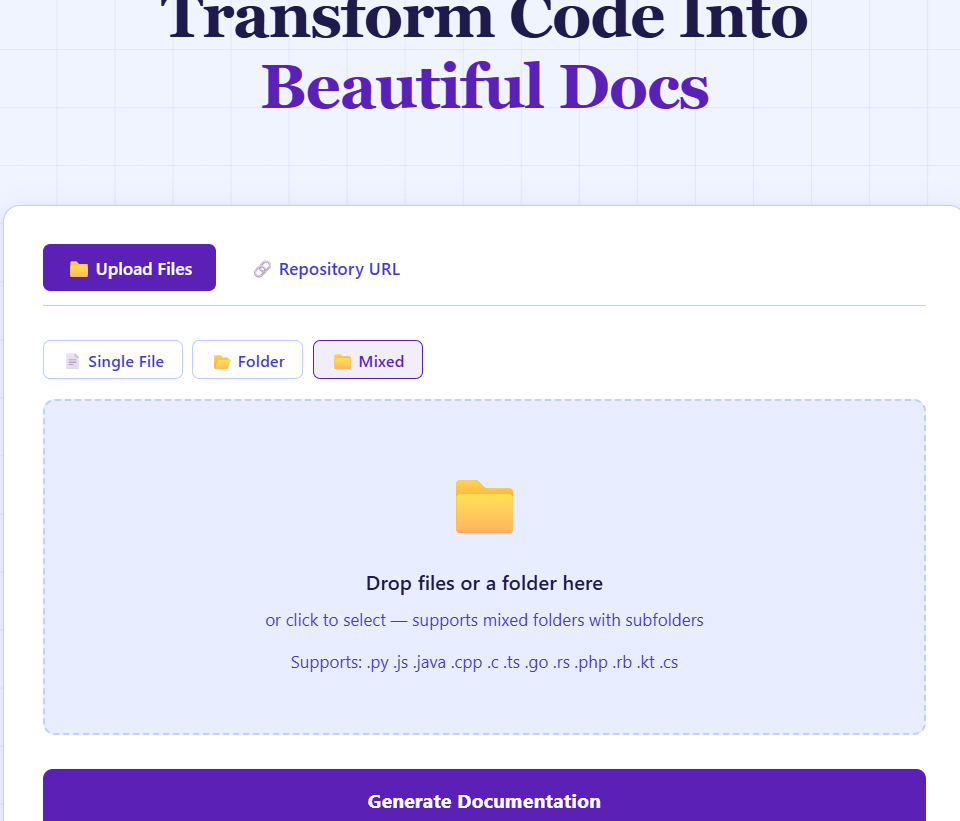
\includegraphics[width=0.6\textwidth]{tex/Screenshot 2026-04-14 215024.png}}
	\caption{Complete User Interface of the System.}
	\label{lvmh2}
\end{figure}
\FloatBarrier

\vspace{1cm}
\begin{figure}[h]
	\centering
	\fbox{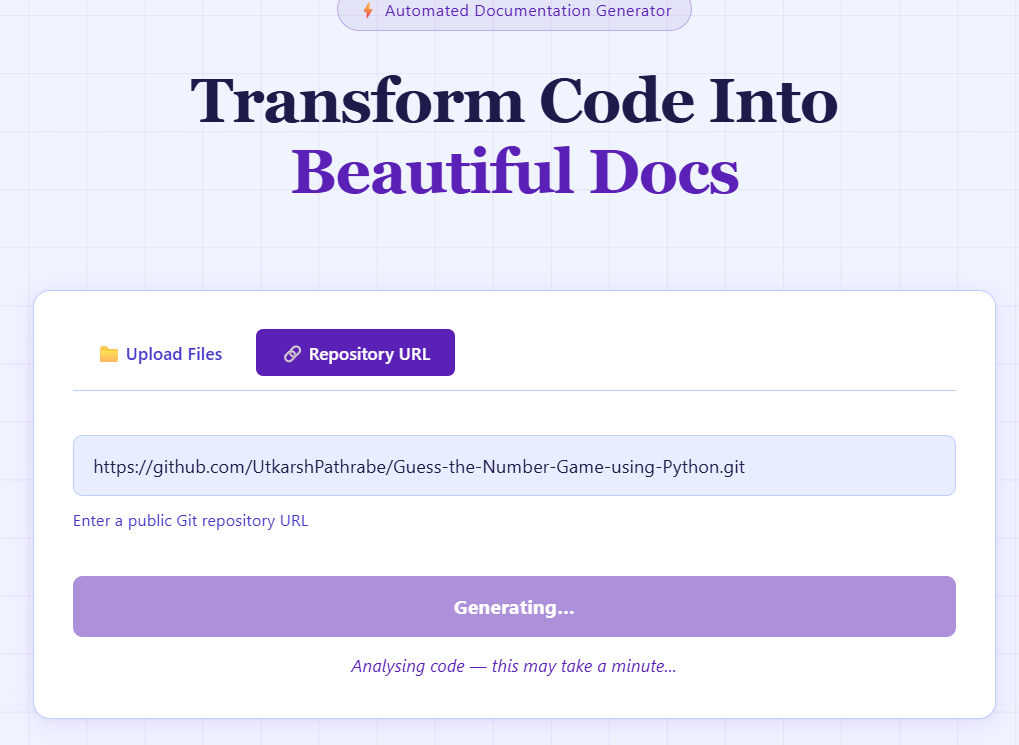
\includegraphics[width=0.6\textwidth]{tex/Screenshot 2026-04-16 072516.png}}
	\caption{Home Page – Repository URL Input Mode.}
	\label{lvmh2}
\end{figure}
\FloatBarrier

\par Figure 7.2 shows the User Interface (UI) for the homepage with the Repository URL mode selected. The user can provide the public git repository URL in the text box. The system then downloads the repository in a temporary directory and processes all the source files from the repository without the need to upload the files.

\vspace{1cm}
\FloatBarrier
\begin{figure}[h]
	\centering
	\fbox{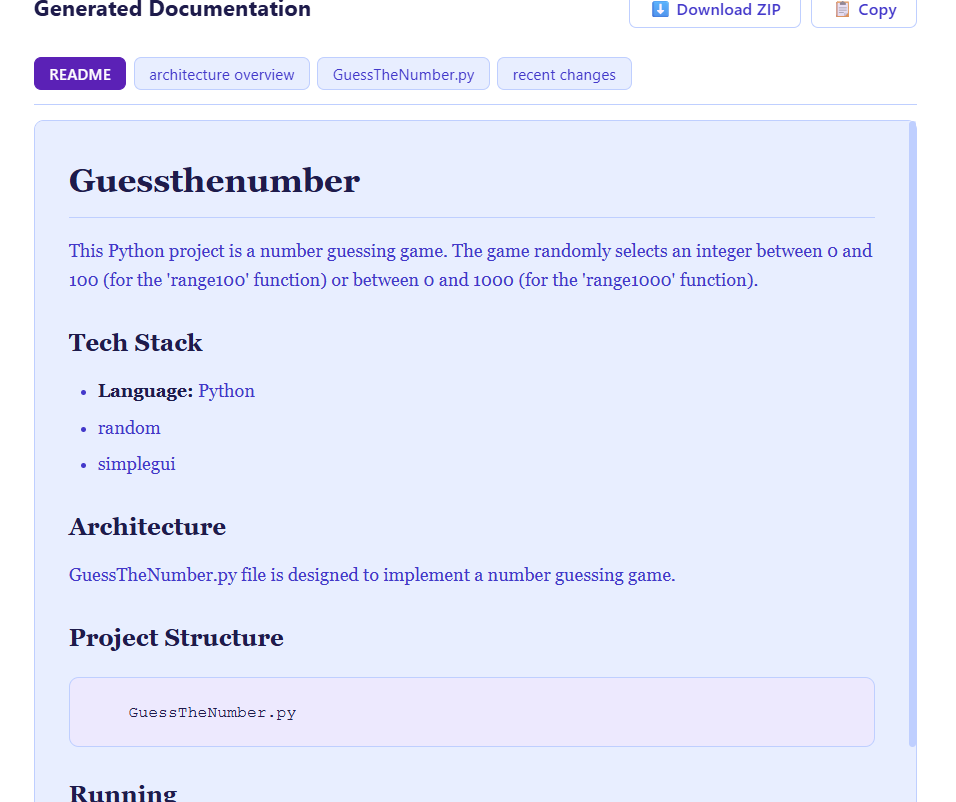
\includegraphics[width=0.6\textwidth]{tex/Screenshot 2026-04-16 073000.png}}
	\caption{README.md – Project Overview Output.}
	\label{lvmh2}
\end{figure}
\FloatBarrier

\par The system shows the README tab of the generated documentation output in Figure 7.3. It analyzes the repository and provides a project-level summary, including project description, technology stack, architecture summary, run instructions, and project structure.

\vspace{1cm}
\FloatBarrier
\begin{figure}[h]
	\centering
	\fbox{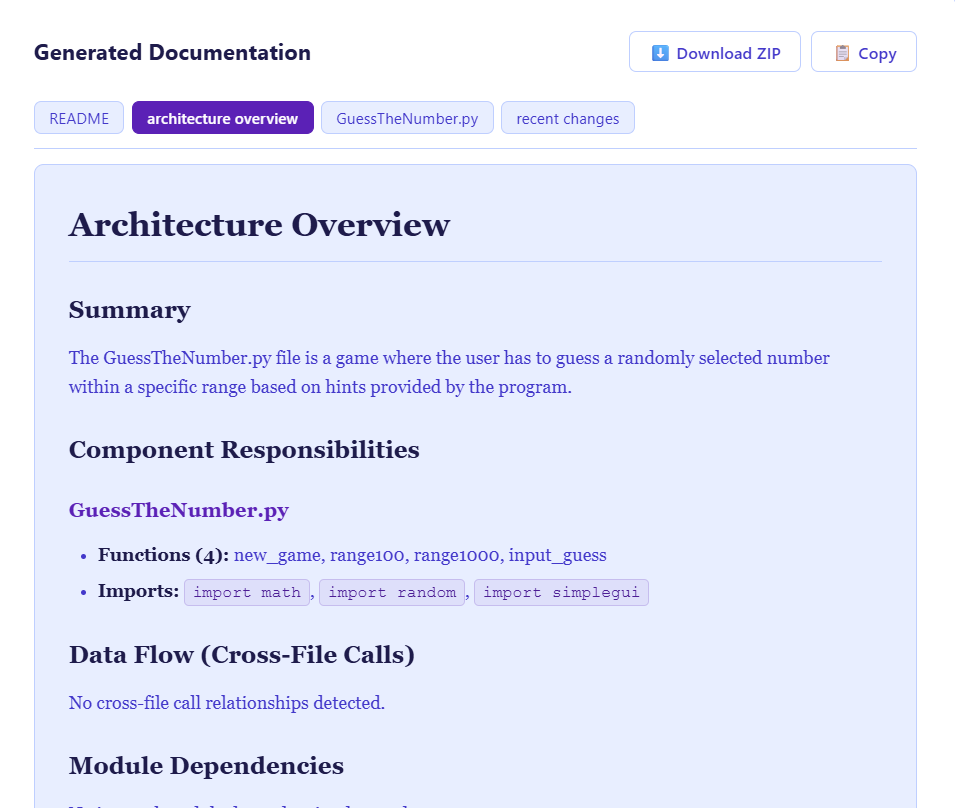
\includegraphics[width=0.6\textwidth]{tex/Screenshot 2026-04-16 073016.png}}
	\caption{architecture\_overview.md – Architectural Description Output.}
	\label{lvmh2}
\end{figure}
\FloatBarrier

\par Figure 7.4 shows the system displaying the Architecture Overview tab of the automatically generated documentation. The system generates a structured architectural description consisting of file-wise summary information, component responsibilities such as classes, functions, imports and fields, call relationships between files representing data flow and module dependencies from both import statements and function interactions.

\par Figure 7.5 shows the file-wise documentation generated for the application in Markdown format. Each file has its documentation with information like function intent, parameters, return values, function calls, local variables and internal call relationships, along with graph-based information like entry points, unused functions, dependencies and recursion information.

\vspace{1cm}
\FloatBarrier
\begin{figure}[h]
	\centering
	\fbox{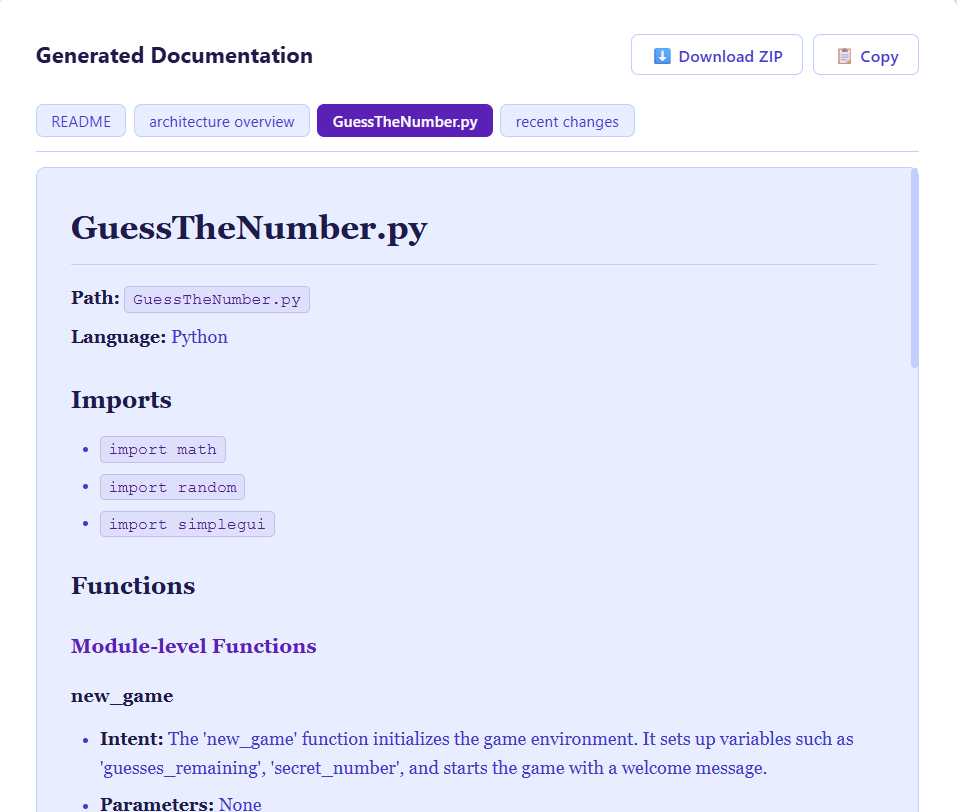
\includegraphics[width=0.6\textwidth]{tex/Screenshot 2026-04-16 073038.png}}
	\caption{File-wise .md Output.}
	\label{lvmh2}
\end{figure}
\FloatBarrier

\par Figure 7.6 shows the Recent Changes tab of the automatically generated documentation. The system has automatically collected the commit history from the Git repository and created a structured document named recent\_changes.md. This feature helps users easily track project updates and understand the evolution of the codebase over time.

\vspace{1cm}
\FloatBarrier
\begin{figure}[h]
	\centering
	\fbox{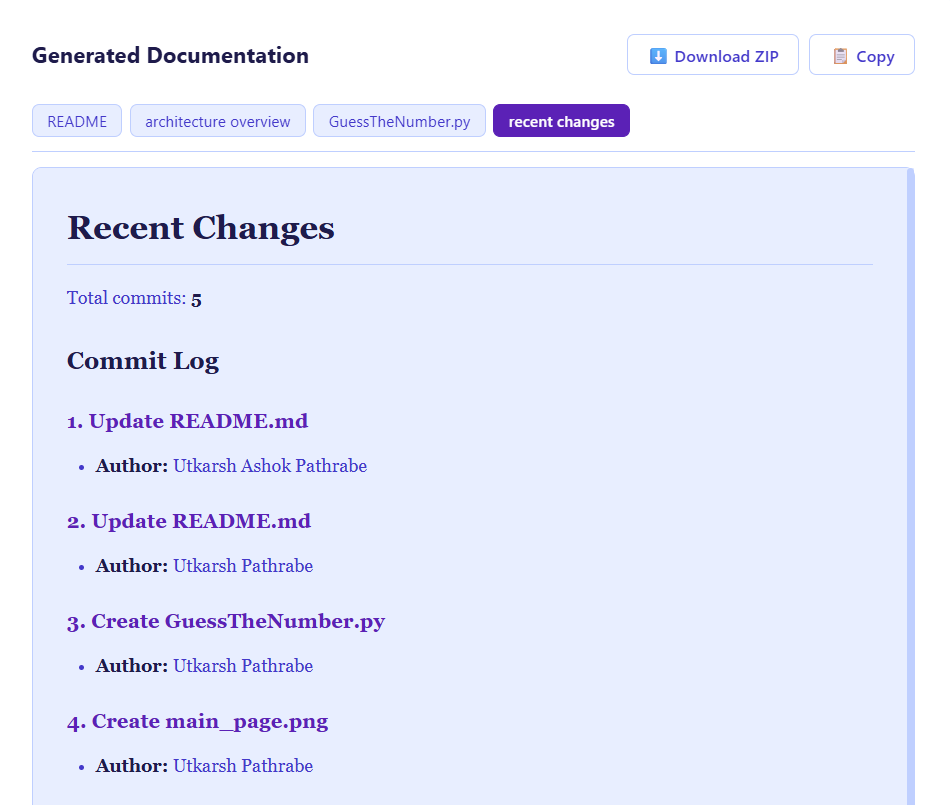
\includegraphics[width=0.6\textwidth]{tex/Screenshot 2026-04-16 073053.png}}
	\caption {recent\_changes.md – Git Commit History Output.}
	\label{lvmh2}
\end{figure}
\FloatBarrier

\section{Discussion}
\hspace{0.5cm}
The results show that the proposed system can efficiently produce overall documentation on different levels, including projects, architecture and functions. The accuracy in the extraction of structural information is guaranteed by AST-based analysis, while graph-based analysis allows for precise identification of relationships between functions. The inclusion of text-based metrics improves the results produced by the system, enhancing their overall relevance and readability.

\par The system works effectively with different programming languages, thus demonstrating the flexibility of the tool. This is further evidenced by the repository URL mode, which is beneficial since the entire projects can be analyzed without the need for file handling. Furthermore, the inclusion of the history of commits is advantageous since it provides additional information compared to other documentation tools.

\par However, the system is not without certain limitations. The quality of the code fed into the system will affect the quality of the documentation that is created. Also, the dynamic behavior of the code is not fully taken into consideration in the system. Nevertheless, the system is useful in reducing the effort required in understanding the code.

% The following figure shows the evaluation of reference audio and test audio by aligning note sequences of both. The green-colored notes represent correct notes. The blue-colored notes are the notes in reference audio missed by test audio. The red-colored notes represent the wrong notes in the test audio. 
% \vspace{1cm}
% \FloatBarrier
% \begin{figure}[h]
% 	\centering
% 	\fbox{\includegraphics[scale=.27]{image/r6.png}}
% 	\caption{Evaluated Notes sequences}
% 	\label{lvmh2}
% \end{figure}
% \FloatBarrier
% % In the following figure show the play back of audio piece correspond to the selected note sequence part. the yellow colored notes are selected by user  for playback. when click  on it a play button is displayed. by click play button the play back can be done.
% %  \vspace{1cm}
% % \FloatBarrier
% % \begin{figure}[h]
% % 	\centering
% % 	\fbox{\includegraphics[scale=.27]{image/result7.png}}
% % 	\caption{Result 7}
% % 	\label{lvmh2}
% % \end{figure}
% % \FloatBarrier
% In the following figure, two play buttons are displayed to playback audio of selected note sequence pieces.
% \vspace{1cm}
% \FloatBarrier
% \begin{figure}[h]
% 	\centering
% 	\fbox{\includegraphics[scale=.27]{image/r7.png}}
% 	\caption{display play buttons on select note sequence peice}
% 	\label{lvmh2}
% \end{figure}
% \FloatBarrier

% % \vspace{1cm}
% % \FloatBarrier
% % \begin{figure}[h]
% % 	\centering
% % 	\fbox{\includegraphics[scale=.27]{image/r8.png}}
% % 	\caption{play back of reference audio}
% % 	\label{lvmh2}
% % \end{figure}
% \FloatBarrier
% The following figure demonstrates inputting reference audio by recording audio using the record button displayed on the interface. Similarly, the test audio can also be recorded in the same manner.
% \vspace{1cm}
% \FloatBarrier
% \begin{figure}[h]
% 	\centering
% 	\fbox{\includegraphics[scale=.27]{image/r9.png}}
% 	\caption{Record reference audio}
% 	\label{lvmh2}
% \end{figure}
% \FloatBarrier

% %  \vspace{1cm}
% % \FloatBarrier
% % \begin{figure}[h]
% % 	\centering
% % 	\fbox{\includegraphics[scale=.27]{image/r10.png}}
% % 	\caption{Record Test audio}
% % 	\label{lvmh2}
% % \end{figure}
% % \FloatBarrier

% % \vspace{1cm}
% % \FloatBarrier
% % \begin{figure}[h]
% % 	\centering
% % 	\fbox{\includegraphics[scale=.27]{image/r11.png}}
% % 	\caption{Note sequence alignment of audio recordings}
% % 	\label{lvmh2}
% % \end{figure}
% % \FloatBarrier
% The following figure shows the time details of notes from audio inputs. 
% \vspace{1cm}
% \FloatBarrier
% \begin{figure}[h]
% 	\centering
% 	\fbox{\includegraphics[scale=.27]{image/r12.png}}
% 	\caption{Display note time sequence}
% 	\label{lvmh2}
% \end{figure}
% \FloatBarrier
% The following figure shows the time duration details of notes and alignment between note sequences from audio inputs.
% \vspace{1cm}
% \FloatBarrier
% \begin{figure}[h]
% 	\centering
% 	\fbox{\includegraphics[scale=.27]{image/r13.png}}
% 	\caption{Display aligned note time sequence}
% 	\label{lvmh2}
% \end{figure}
% \FloatBarrier
% The following figure shows the alignment between note sequences by removing time duration from audio inputs.
%  \vspace{1cm}
% \FloatBarrier
% \begin{figure}[h]
% 	\centering
% 	\fbox{\includegraphics[scale=.27]{image/r14.png}}
% 	\caption{Display aligned note sequence}
% 	\label{lvmh2}
% \end{figure}
% \FloatBarrier
% \subsection{Accuracy in note sequence detection}
% The table below illustrates the accuracy of note sequence detection across various guitar audio recordings.
% \begin{table}[h]
%     \centering
%     \begin{tabular}{|c|c|c|c|}
%         \hline
%          \multirow{2}{*}{}  & Actual note & Detected note &   \\
%           & sequence & sequence & Match \\ 
%         % \thead{ } & \thead{Pitch, onset,\\ & and offset}  & \thead{Pitch and onset} & \thead{Onset only} & \thead{Offset only} \\
%         \hline
%         Guitar Audio 1 & M4 n4	D4	n4 P4 G4 & M4 n4	D4	n4 P4 G4 & \\
%         & D4	P4 M4	D4	M4 & D4	P4 M4	D4	M4 & 100\%\\
%         \hline
%          Guitar Audio 2 & M4 S5	N4	S5 D4   & M4 S5	N4	S5 D4 & \\
%         & N4 D4 M4 D4 P4 & N4 D4 M4 D4 P4 & \\
%          &  M4 G4 P4 & M4 G4 P4 & 100\%\\
%         \hline
%          Guitar Audio 3 & G4	 g4 G4 g4 m4    & G4	 g4 G4 g4 m4 & \\
%         & g4 m4 g4 m4 d4 & g4 m4 g4 m4 d4 & \\
%          &  D4 m4 g4  & D4 m4 g4 & 100\%\\
%         \hline
%          Guitar Audio 4 & d4 n4	D4	p4 P4 & d4 n4	D4	p4 P4 & \\
%         & g4	P4 M4 r4	M4 & g4	P4 M4 r4	M4 & 100\%\\
%         \hline
%          Guitar Audio 5 & s4 r4	G4	m4 P4  & s4 r4	G4	m4 P4 & \\
%           & m4 n4	G4	r4 G4  & m4 n4	G4	r4 G4 & \\
%         & D4 P4 M4	G4	r4 &  D4 P4 M4	G4	r4 & 100\%\\
%         \hline
%     \end{tabular}
%     \caption{Accuracy in detected note sequence of guitar music}
%     \label{tab:simple_table}
% \end{table}
% The table below illustrates the accuracy of note sequence detection across various piano audio recordings.
% \begin{table}[h]
%     \centering
%     \begin{tabular}{|c|c|c|c|}
%         \hline
%          \multirow{2}{*}{}  & Actual note & Detected note &   \\
%           & sequence & sequence & Match \\ 
%         % \thead{ } & \thead{Pitch, onset,\\ & and offset}  & \thead{Pitch and onset} & \thead{Onset only} & \thead{Offset only} \\
%         \hline
%         Guitar Audio 1 & M4 n4	D4	n4 P4 G4 & M4 n4	D4	n4 P4 G4 & \\
%         & D4	P4 M4	D4	M4 & D4	P4 M4	D4	M4 & 100\%\\
%         \hline
%          Guitar Audio 2 & M4 S5	N4	S5 D4   & M4 S5	N4	S5 D4 & \\
%         & N4 D4 M4 D4 P4 & N4 D4 M4 D4 P4 & \\
%          &  M4 G4 P4 & M4 G4 P4 & 100\%\\
%         \hline
%          Guitar Audio 3 & G4	 g4 G4 g4 m4    & G4	 g4 G4 g4 m4 & \\
%         & g4 m4 g4 m4 d4 & g4 m4 g4 m4 d4 & \\
%          &  D4 m4 g4  & D4 m4 g4 & 100\%\\
%         \hline
%          Guitar Audio 4 & d4 n4	D4	p4 P4 & d4 n4	D4	p4 P4 & \\
%         & g4	P4 M4 r4	M4 & g4	P4 M4 r4	M4 & 100\%\\
%         \hline
%          Guitar Audio 5 & s4 r4	G4	m4 P4  & s4 r4	G4	m4 P4 & \\
%           & m4 n4	G4	r4 G4  & m4 n4	G4	r4 G4 & \\
%         & D4 P4 M4	G4	r4 & D4 P4 M4	G4	r4 & 100\%\\
%         \hline
%     \end{tabular}
%     \caption{Accuracy in detected note sequence of piano music}
%     \label{tab:simple_table}
% \end{table}
%  To assess the accuracy of note sequences, several piano and guitar audio recordings were examined, revealing a 100\% accuracy rate. However, identifying the actual note sequence in vocal audio poses challenges due to variations in voice tone. But we can expect the note sequence of vocal audio. Here, the detected note sequence is also evaluated based on the expected note sequence. It provides accuracy of more than 80\% in vocal audio note sequence detection. If the audio is noise-free then it can provide 100\% accuracy. The proposed system can be used only for monophonic audio.
%  \subsection{ Result of Note sequence alignment}
%  The proposed Dynamic Time Warping algorithm has optimally aligned the note sequence, obtaining the maximum matching between note sequences. It accurately shows mistakes in test notes and provides a match score. Since the Dynamic Time Warping algorithm uses dynamic programming, its accuracy is 100\%.
% \par
% Figure 7.1 depicts the home page of the application. On the left side of the page, there are three buttons, while a frame is positioned on the right. The content within the frame dynamically changes according to the buttons clicked on the left side of the page. The first button name with \textbf{Create Tune} navigates to the tune creation process, the second button name with \textbf{Play Tune} leads to the tune playback process, and the third button name with \textbf{Convert to audio} directs to the audio conversion process.  
% \FloatBarrier
% \begin{figure}[h]
% 	\centering
% 	\fbox{\includegraphics[scale=.26]{image/result3.png}}
% 	\caption{Raga Selection}
% 	\label{lvmh2}
% \end{figure}
% \FloatBarrier

% Figure 7.2 shows the raga selection process initiated upon clicking the \textbf{Create Tune} button. It displays 72 raga options for selection. Upon choosing a raga, the interface navigates to another page, as represented in Figure 7.3. 



% \FloatBarrier
% \begin{figure}[h]
% 	\centering
% 	\fbox{\includegraphics[scale=.26]{image/result5.png}}
% 	\caption{Virtual Keyboard}
% \end{figure}
% \FloatBarrier

% \par Figure 7.3 demonstrates the presentation of a virtual keyboard corresponding to the selected raga. Each key on the virtual keyboard is associated with microtones of notes, concurrently mapped with the system keyboard labeled from 1 to 9. This interface enables the creation of note sequences. Additionally, this page offers options to customize instrument sounds, a button for tune replay, a slider to adjust speed, as well as buttons to save or discard tunes. When the 'Save' button is clicked, it prompts the user to enter a file name.

% \FloatBarrier
% \begin{figure}[h]
% 	\centering
% 	\fbox{\includegraphics[scale=.26]{image/result7.png}}
% 	\caption{Playback Tune}
% \end{figure}
% \FloatBarrier

% \par Figure 7.4 demonstrates the tune-playing process initiated upon clicking the \textbf{Play Tune} button. This interface provides an input feature to upload a sequence file to play and offers options to customize instrument sounds, a button for tune play, and a slider to adjust speed.

% \FloatBarrier
% \begin{figure}[h]
% 	\centering
% 	\fbox{\includegraphics[scale=.26]{image/result9.png}}
% 	\caption{Input sequence file for audio conversion}
% \end{figure}
% \FloatBarrier
% % \par In figure 7.5, the same person's ECG is taken in a different date.

% % \FloatBarrier
% % \begin{figure}[h]
% % 	\centering
% % 	\fbox{\includegraphics[scale=.27]{image/result11.png}}
% % 	\caption{Sample Output 2}
% % \end{figure}
% % \FloatBarrier
% \par Figure 7.5 demonstrates the audio converting process initiated upon clicking the \textbf{Convert to Audio} button. This interface provides an input feature to upload a sequence file to convert into audio and offers options to customize instrument sounds, a button name with \textbf{Make Audio file}, and a slider to adjust speed. Upon clicking the \textbf{Make Audio file} button, the interface navigates to another page, as represented in Figure 7.6. 
% \FloatBarrier

% \begin{figure}[h]
% 	\centering
% 	\fbox{\includegraphics[scale=.26]{image/result10.png}}
% 	\caption{sequence file to audio conversion}
% \end{figure}
% \FloatBarrier
% \par Figure 7.6 illustrates the outcome after clicking the \textbf{Make Audio file} button. The  \textbf{Play} button enables previewing of the converted audio, and the  \textbf{Download} button allows users to download it. Upon clicking the \textbf{Download} button, the interface prompts the user to enter a file name, as represented in Figure 7.7. 

% \FloatBarrier
% \begin{figure}[h]
% 	\centering
% 	\fbox{\includegraphics[scale=.26]{image/result12.png}}
% 	\caption{Downloading audiofile}
% \end{figure}
% \FloatBarrier
% \textbf{Result:} All the functionalities provided in the system, such as raga selection, instrument selection, playback speed adjustment, playing tunes from sequence files, and audio conversion, are operating smoothly. The tune played from the sequence file achieves a 100\% accuracy rate. The audio obtained after converting the sequence file to an audio file precisely matches the played tune.

% \chapter{Evaluation and Results}

%\section{Performance Evaluation}
% \subsection{Evaluation Result}

% \subsubsection{Field Extraction Accuracy}
% Field extraction was carried out using a combination of libraries such as \texttt{pdfplumber} for digital PDFs and \texttt{pytesseract} with preprocessing techniques (binarization, noise removal, thresholding) for scanned images. The extracted text was cleaned and normalized using regular expressions and \texttt{numpy}.  

% For digital PDFs, the system extracted most fields accurately. Aadhaar numbers from Digilocker PDFs appeared masked (e.g., \texttt{XXXX XXXX 1234}), and Driving License numbers were extracted correctly but without spacing between the regional code and number (e.g., \texttt{KL089875678229} instead of \texttt{KL08 9875678229}). In rare cases (1 out of 8), the Aadhaar Name field concatenated with the address label due to formatting inconsistencies. Other fields such as Date of Birth, Gender, Address, SGPA, and Percentage were extracted with full accuracy.  

% When a scanned Aadhaar image (JPEG) was uploaded in addition to the PDFs, the full Aadhaar number was extracted successfully, and the Name concatenation issue was avoided, improving overall accuracy.  

% % \begin{table}[H]
% % \centering
% % \caption{Field-wise Accuracy (PDFs only)}
% % \begin{tabular}{|l|c|l|}
% % \hline
% % \textbf{Field} & \textbf{Accuracy} & \textbf{Remarks} \\ \hline
% % Name & 87--88\% & Correct in most cases. \\ \hline
% % Date of Birth & 100\% & Consistently extracted. \\ \hline
% % Gender & 100\% & Extracted from Aadhaar. \\ \hline
% % Aadhaar Number & 50\% & Masked in Digilocker PDFs  \\ \hline
% % PAN Number & 100\% & Fully extracted. \\ \hline
% % Driving License Number & $\sim$95\% & Value correct; spacing issue present. \\ \hline
% % Address & 100\% & Extracted reliably. \\ \hline
% % SGPA & 100\% & Extracted from marklists. \\ \hline
% % Percentage & 100\% & Extracted from marklists. \\ \hline
% % \end{tabular}
% % \end{table}

% \noindent Overall field extraction accuracy with only PDFs was approximately \textbf{88--90\%}, with main limitations being the masked Aadhaar number, minor formatting inconsistencies in Driving License numbers, and rare concatenation of Aadh-aar Name with Address.
% \subsection{Field Extraction Accuracy}
% \hspace{0.5cm} Field extraction used \texttt{pdfplumber} for digital PDFs and \texttt{pytesseract} with preprocessing (binarization, noise removal, thresholding) for scanned images. Text was cleaned and normalized with regular expressions and \texttt{numpy}.  

% Most fields were accurately extracted from PDFs. Aadhaar numbers from Digilocker PDFs were masked (e.g., \texttt{XXXX XXXX 1234}) and Driving License numbers lacked spacing (e.g., \texttt{KL089875678229}). Rarely, the Aadhaar Name concatenated with the address. Other fields, including Date of Birth, Gender, Address, SGPA, and Percentage, were fully extracted.  

% Adding scanned Aadhaar images resolved masking and concatenation issues. Overall field extraction accuracy with PDFs alone was around \textbf{88--90\%}, with minor limitations due to masked Aadhaar numbers and formatting inconsistencies.



% \subsection{Consolidated Profile Accuracy}
% \hspace{0.3cm} The consolidation step merged extracted fields from multiple documents into a unified profile. Conflicts (e.g., different spellings of a name or minor formatting differences) were resolved using frequency-based selection and semantic similarity matching with \texttt{sentence-transformers}.  
% Across all tested cases, the system achieved \textbf{100\% consolidation accuracy}, producing reliable profiles.

% \subsection{Form Auto-Filling Accuracy}
% \hspace{0.3cm} For form filling, extracted fields were mapped to target form fields using semantic similarity techniques. Even when labels in the form were phrased differently (e.g., ``DOB'' vs ``Date of Birth''), the model correctly identified matches. The auto-fill module then populated the fields using Python browser automation.  
% In testing with 16 expected form fields, the system filled all fields correctly, resulting in a \textbf{100\% form filling accuracy}.

% \subsection{User Verification and Correction Rate}
% \hspace{0.3cm} Once the form was auto-filled, users could review the results. Since the system’s accuracy was very high, manual corrections were rarely required. For digital PDFs alone, Aadhaar numbers required correction due to masking, and the occasional Name concatenation had to be fixed. With supporting Aadhaar images provided, no manual corrections were necessary, except for minor adjustments in the Driving License number formatting.  
% This gives the system an effective correction rate of \textbf{0--2\%}, showing strong reliability.

% \subsubsection{Processing Time}
% The system processed digital PDFs efficiently, completing extraction and form filling in an average of \textbf{3--5 seconds} for four documents. When scanned images were included, the time increased slightly due to OCR preprocessing, averaging \textbf{5--7 seconds}, which is still acceptable for practical use. 
% \subsection{Processing Time}
% \hspace{0.3cm} The system processed digital PDFs efficiently, completing extraction and form filling in an average of \textbf{3--5 seconds} for four documents. When scanned images were included, the time increased slightly due to OCR preprocessing, averaging \textbf{5--7 seconds}. These times were measured by recording the duration from the moment documents were uploaded to the point when the form was fully autofilled, using Python's built-in timing functions, which provides a practical estimate of real-world performance.

% \newpage
% \subsection{Observations}
% \begin{itemize}
%     \item Digital PDFs achieved high accuracy, but Aadhaar numbers were masked in Digilocker files.
%     \item In 1 of 8 cases, the Aadhaar Name field concatenated with the Address, slightly reducing accuracy.
%     \item Adding scanned Aadhaar images resolved masking and name concat-enation, improving accuracy to nearly 100\%.
%     \item Driving License numbers were correct but spacing inconsistencies slightly reduced accuracy.
%     \item The auto-filling module demonstrated robustness by correctly mapping fields even with inconsistent naming.
%     \item Minimal user corrections were required, confirming the system’s efficie-ncy and practicality.
% \end{itemize}

% \subsection*{\hspace{-0.1cm}Observations}
% \begin{itemize}
%     \item Digital PDFs were generally accurate, though Aadhaar numbers were masked.
%     \item Rarely, Aadhaar Name concatenated with the Address, slightly reducing accuracy.
%     \item Adding scanned Aadhaar images resolved masking and concatenation issues.
%     \item Driving License numbers had minor spacing inconsistencies.
%     \item Auto-filling correctly mapped fields even with inconsistent naming.
%     \item Minimal user corrections were needed, confirming system reliability.
% \end{itemize}
